\section{Exercise 4}
A sensor records the following values given as pair  in file data.dat.
Read in the data using numpy's loadtxt package and perform the following:

\subsection{Part a.}
Using Python, plot the measurements at their corresponding time on a
graph.
\begin{mdframed}[style=MyFrame]
    The following plot represents the scatter plot for the velocities
    and the corresponding times.
    \begin{figure}[H]
        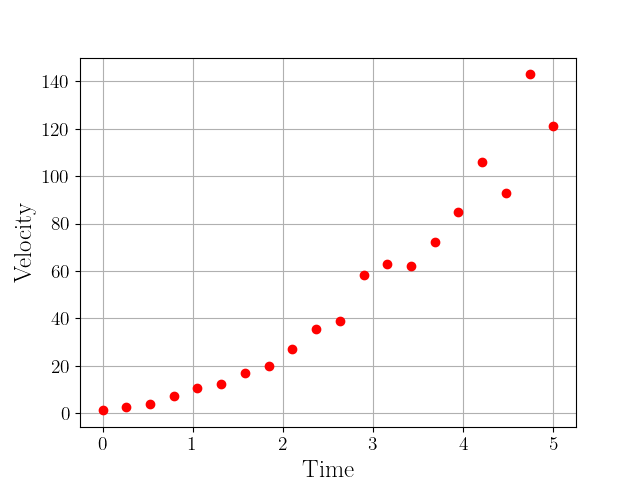
\includegraphics[height=0.35\textheight]{media/scatter.png}
        \caption{Velocity vs. time}
    \end{figure}
\end{mdframed}

\subsection{Part b.}
Find the line that best fits the data and plot it on your graph. What is
the least square error?
\begin{mdframed}[style=MyFrame]
    The line of best fit is found by fitting the data to a linear line,
    \begin{equation}
        u = At + B
        \label{eq:linear-4}
    \end{equation}
    This gives
    \begin{equation}
        \mathbf{A}
        \begin{bmatrix}
            A   \\
            B
        \end{bmatrix}
        = \mathbf{u}
    \end{equation}
    where $\mathbf{A}$ is a $M \times 2$ matrix containing the RHS of
    Eq.~(\ref{eq:linear-4}). Next we can solve for the coefficients
    $A$ and $B$ using the least squares method,
    \begin{equation}
        \widehat{\mathbf{x}} = 
            \left(\mathbf{A}^{T} \mathbf{A}\right)^{-1} \mathbf{A}^{T}
            \mathbf{b}
    \end{equation}
    Solving we get the following equation,
    \begin{equation}
        u(t) = 26.5t - 17.2
    \end{equation}
    and the following plot
    \begin{figure}[H]
        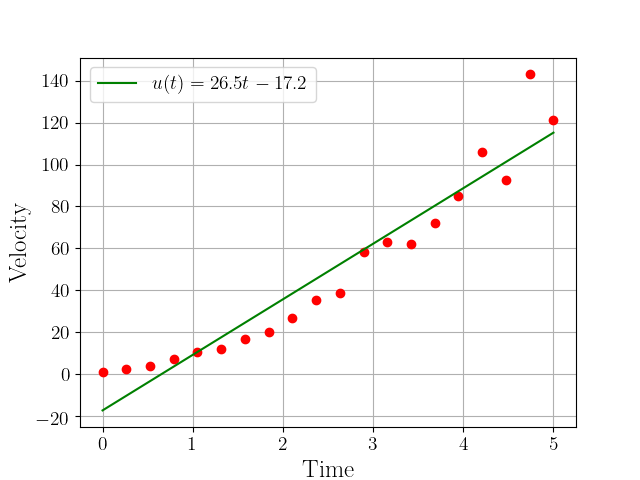
\includegraphics[height=0.35\textheight]{media/linear.png}
        \caption{Linear approximation using least squares method}
    \end{figure}
    Furthermore, we can find the least squares error using the following 
    \begin{equation}
        E^{2} = \sum_{i=1}^{N} e_{i}^{2}
    \end{equation}
    where,
    \begin{equation}
        \mathbf{e} = \mathbf{b} - \mathbf{A} \mathbf{\widehat{x}}
    \end{equation}
    Using the solution to linear it we get a least squares error of
    $E=53.54$.
\end{mdframed}

\subsection{Part c.}
Find a parabola that best fits the data. Which curve best fits the data?
\begin{mdframed}[style=MyFrame]
    We can repeat the process and fit the data to a parabola
    using, 
    \begin{equation}
        u(t) = At^{2} + Bt + C
        \label{eq:parabolic}
    \end{equation}
    where $\mathbf{A}$ is a $M \times 3$ matrix containing the RHS of
    Eq.~(\ref{eq:parabolic}).
    Solving we get the following equation and plot,
    \begin{equation}
        u(t) = 4.5t^{2} + 3.8t + 0.7
    \end{equation}
    \begin{figure}[H]
        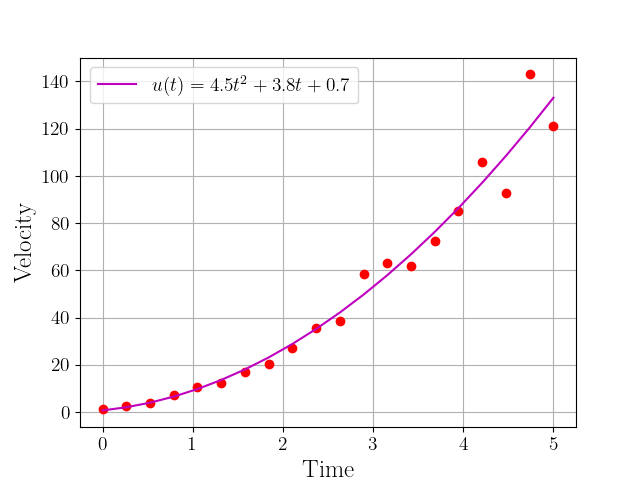
\includegraphics[height=0.35\textheight]{media/parabolic.png}
        \caption{Parabolic approximation using least squares method}
    \end{figure}
    Lastly, we can calculate the least squares error giving $E=33.75$,
    therefore the parabolic data best fits the velocity data. 
\end{mdframed}
\emph{\textbf{Please see the attached code in the Appendix}}
